
\subsection{Uncertain Injects}
\bc{\begin{frame}{Uncertain Injects}
\alert{Uncertainty in Injects to Power System}
\bi
\item Subset of nodes have uncertain injections
\bi
\item Solar, wind
\item Demand (relatively certain, however EVs could represent change)
\ei
\pause
\item Subset of assets respond to uncertainty (slack distribution)
\bi
\item Rotational inertia, peaker plants and regulation
\item Energy storage, enhanced power controls
\ei
\ei
\end{frame}
}

\begin{frame}{Uncertainty is Multivariate Normal}
\alert{Assumption}

Uncertainty in net injections are Multivariate Normal
\bi
\item \textit{Uncertainty in errors from forecast}
\item Known or can be empirically estimated
\item Potentially correlated
\ei
\begin{center}
% 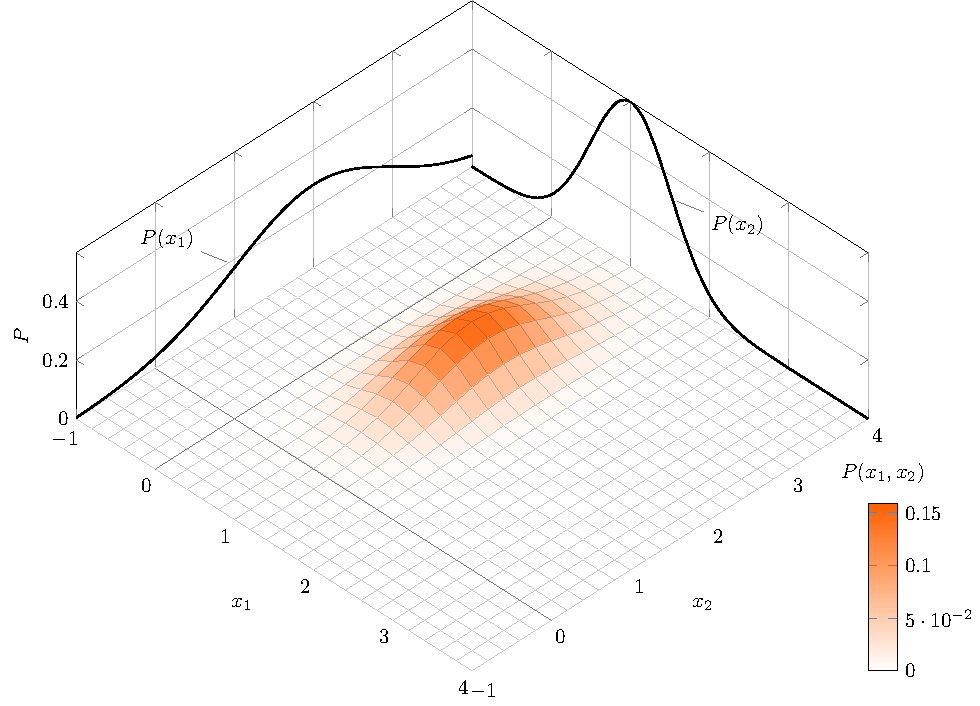
\includegraphics[scale=.325]{multivariate} 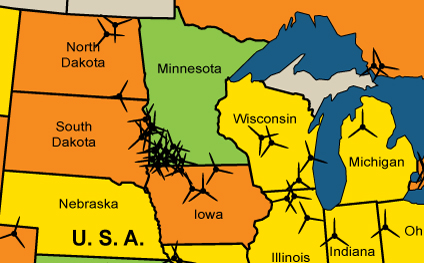
\includegraphics[scale=.35]{windmap}
\begin{figure}
   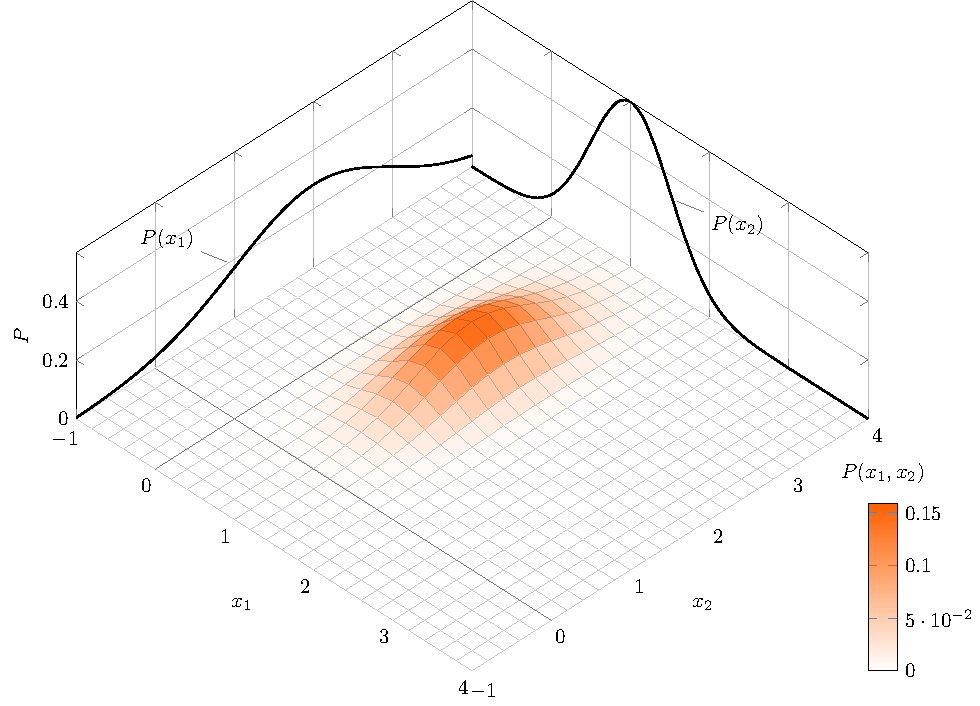
\includegraphics[width=0.475\textwidth]{multivariate}
   \hfill
   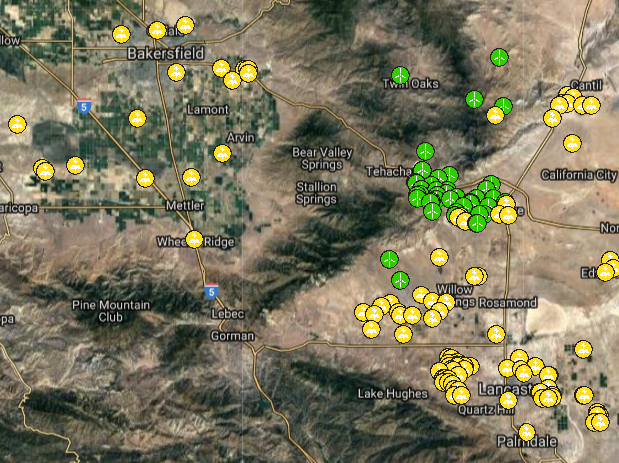
\includegraphics[width=0.475\textwidth]{renewables-correlated}
\end{figure}
\end{center}
%Error from short term forecast for windfarms is normally distributed

\end{frame}



\subsection{Issues with Deterministic Analysis}
\begin{frame}{Issues with Deterministic Analysis}
Normal distributed injects 
\pause 
$\rightarrow $
\textbf{Normal branch flows}\footnotemark
\vspace{20px}
\footnotetext[1]{In a stable system}
\pause
\alert{Problem!}
\bi
\item Branch constraints violated half the time when at its limit
\ei
\end{frame}

\begin{frame}{Normal Branch Flow}
\begin{center}
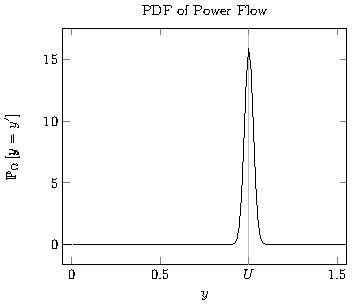
\includegraphics[scale=1.1]{\mypathjcc/fig-ccflow}
\end{center}
PDF for Branch flow with mean (forecast) at nominal capacity
\end{frame}


\begin{frame}{Normal Branch Flow}
\begin{center}
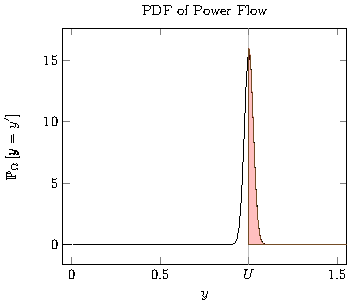
\includegraphics[scale=1.1]{\mypathjcc/fig-ccflowred}
\end{center}

\alert{Need to probabilistically enforce constraints}

\end{frame}


\subsection{Chance Constraints}
\begin{frame}{Chance Constraints}

\begin{center}
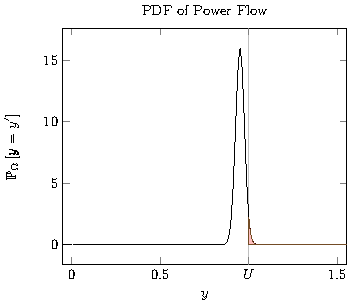
\includegraphics[scale=1.1]{\mypathjcc/fig-ccflowred-95}
\end{center}


\end{frame}

\subsection{System Risk}
\begin{frame}{Current Models}
Determinsitic has fixed line thresholds
\bi
\item Line is completely okay
\item or system is infeasible
\ei
\pause
Chance Constraints
\bi
\item Enforce line threshold probalistically
\ei
\pause

\alert{Line thresholds are soft constraints in real life}
\pause
\bi
\item Multiple line ratings (i.e. short term emergency rating)
\item Hard limit typically relay tripping
\ei
\end{frame}

\begin{frame}{Line Limits}
Limited by
\bi
\item Sagging due to current flow and line heating
\item \alert<2>{Worst case environmental conditions (seasonally)}
\item An acceptable probability of line failure
\item Enforce N-1 Reliability Constraint
\ei
\bigskip
\pause
\textbf{Dynamic line limits}
\bi
\item Real time limits based on current environmental conditions
\ei

\end{frame}

\begin{frame}{System Risk}

System risk related to line loadings (severity measure) \footnotemark
%\footfullcite{wang_2013}
\footnotetext[2]{Qin Wang and McCalley, J.D. and Tongxin Zheng and Litvinov, E.}
\pause


\vspace{10pt}
Intuition
\bi
\item Grid relatively stressed when more lines are near their limit
\ei
%Want risk measure to compare risk of line loadings
%\vspace{10pt}
\end{frame}
\begin{frame}{Line Failure Model}

Model for line failure risk

\begin{center}
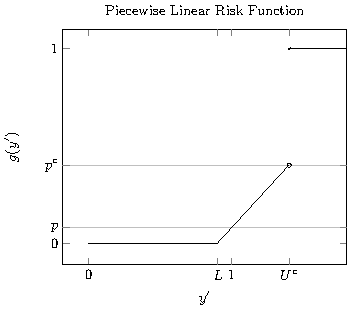
\includegraphics[scale=0.7]{\mypathjcc/fig-failuredensity}
\end{center}
\pause

Individual lines contribute to system risk
\bi
\item Balance economic object with system risk
\item Cost-risk frontier
\ei
%\vspace{50pt}
%This is the product of the probability that each line does not fail
%\begin{equation*}  
%h(y) = \prod_{e \in \cE} \left( 1 - g(y_e) \right)
%\end{equation*}  
%\bi
%\item Implies hard line constraint, line risk=system risk
%\ei
%In the static case
%\bi
%\item Perform log transform to get exact solution
%\ei

\end{frame}



% \begin{frame}{Line Risk Function}
% Risk function takes the normalized flow returns line risk 
% \begin{equation*}
%  g(\hy_e) = \bP{\Xi}{\text{Line }e\text{ fails} | \hy_e} 
% \end{equation*}
% \pause
% Piece-wise linear function choosen
% \bi
% \item Below $L$, there is no risk associated with loading
% \item After $L$, the risk increases linearly with loading
% \item At critical capacity $U^c$, line fails with certainty
% \ei
% \pause
% \begin{equation*}
% g(\hy_e) = \left\{ \begin{array}{l l}
%   0 & \hy_e \leq L \\
%   a + b \hy_e & L \leq \hy_e < U^c \\
%   1 & U^c \leq \hy_e 
% \end{array}
% \right.
% \end{equation*}
% \end{frame}

%\begin{frame}{Gaussian Branch Flow}
%\begin{center}
%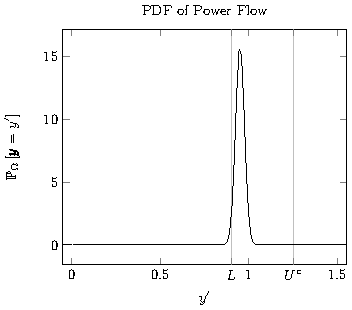
\includegraphics[scale=1.2]{\mypathjcc/fig-pdfflow}
%\end{center}
%\end{frame}

